\documentclass{beamer}
\usepackage[utf8]{inputenc}
\usepackage{amsmath}
\usepackage{amsfonts}
\usepackage{amssymb}

\mode<presentation>
{
	\usetheme{Madrid}       % or try default, Darmstadt, Warsaw, ...
	\usecolortheme{default} % or try albatross, beaver, crane, ...
	\usefonttheme{serif}    % or try default, structurebold, ...
	\setbeamertemplate{navigation symbols}{}
	\setbeamertemplate{caption}[numbered]
} 
\usepackage[english]{babel}


\title{Towards Bayesian Subject Model}
\author{Krzysztof Rusek}
\institute{AGH University of Science and Technology}
\date{\today}




\begin{document}
	
\begin{frame}
\titlepage
\end{frame}


\begin{frame}{Simple subject model }
$$U_{ij}=\psi_{j} + \Delta_i + \upsilon_i X + \phi_{j} Y$$
$$X,Y \sim N(0,1)$$
\begin{block}{Parameters}
	$$\theta = (\psi_{j}, \Delta_i, \upsilon_i ,\phi_j,) $$
\end{block}
\begin{definition}{Maximum likelihood estimator}
	$$\hat \theta = \arg\max_\theta P(u|\theta) $$
\end{definition}

\end{frame}

\begin{frame}{Problems}
\begin{enumerate}
	\item $U_{ij}\in\{1,2,3,4,5\}\nsim N(\psi_{j}+\Delta_i, \sqrt{\upsilon_i^2 +\phi_j^2}) $
	\item Non unique solutions: how to partition variance among testers and PVSs?
\end{enumerate}
\begin{center}
	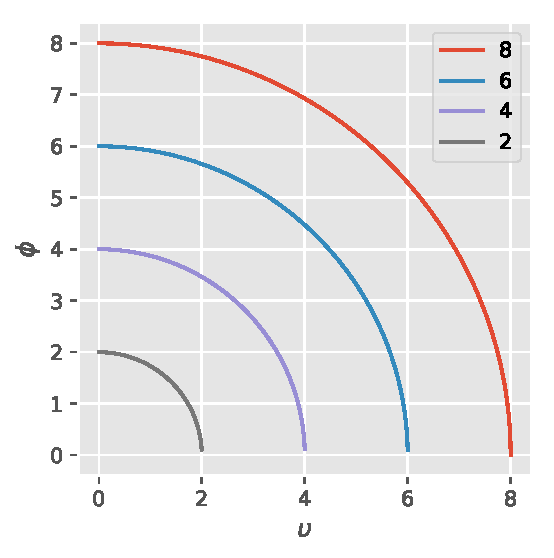
\includegraphics[width=0.4\linewidth]{izovar}
\end{center}

	
\end{frame}

\begin{frame}{Solutions}
	\begin{enumerate}
		\item $U_{ij} \sim Q(N(\psi_{j}+\Delta_i, \sqrt{\upsilon_i^2 +\phi_j^2}) ) $, $Q()$ - a quantizer (e.g ceil)
		\item Use prior knowledge (expert, domain specific, etc) about parameters expressed as distribution.
	
	\end{enumerate}
\begin{example}{Bayesian model}
	\begin{enumerate}
		\item $\upsilon \sim Gamm(\alpha_1,\beta_1)$
		\item $\phi \sim Gamm(\alpha_2,\beta_2)$
		
	\end{enumerate}
\end{example}
\end{frame}

\begin{frame}{Priors}
	\begin{center}
		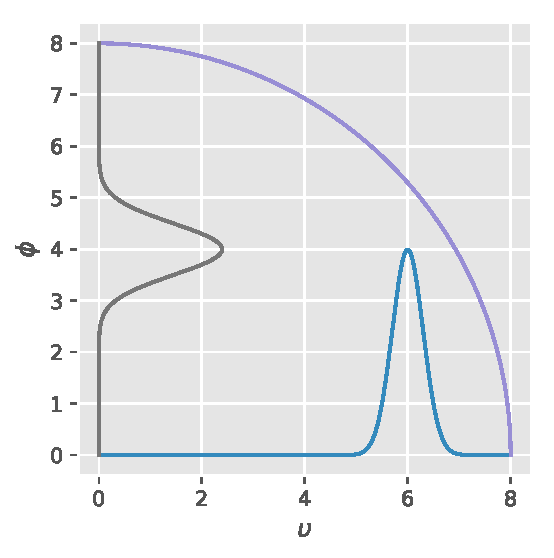
\includegraphics[width=0.6\linewidth]{izovarprior}
	\end{center}
	
\end{frame}

\begin{frame}{Bayesian subject model - not yet}
 \begin{theorem}[Bayes]
  $$P(\theta|u)=\frac{P(u ,\theta )}{P(u)}=\frac{P(u |\theta ) P(\theta)}{P(u)}$$
 \end{theorem}
	
	
	\begin{definition}{Maximum a'posteriori estimator (MAP)}
		$$ \hat \theta = \arg \max_\theta P(\theta|u)$$
	\end{definition}
	\begin{alertblock}{MLE $\rightarrow$ MAP}
		$$
		\log P(\theta|u) = \log P(u |\theta ) + \log P(\theta) - \log P(u)
		$$
		Just add  regularization given by log prior $\log P(\theta)$.
	\end{alertblock}
	

\end{frame}

\begin{frame}{Tensorflow Probability}
	\begin{enumerate}
		\item Based on TensorFlow, R like, GPU Accelerated.
		\item Rich library of distributions (Normal, {\bf QuantizedDistribution} ).
		\item Probabilistic programming language for model building.
		\item Optimizers from TensorFlow for MAP, MLE ($\arg\min_\theta$) 
		\item Designed for Bayesian Inference ( {\bf MCMC}, tbd...).
	\end{enumerate}
\begin{example}
	\url{https://goo.gl/G4XR1C}
\end{example}
\end{frame}
\begin{frame}{}
\begin{center}
	\large
	Results
\end{center}
\end{frame}
\begin{frame}{MLE - continuous}
\begin{center}
	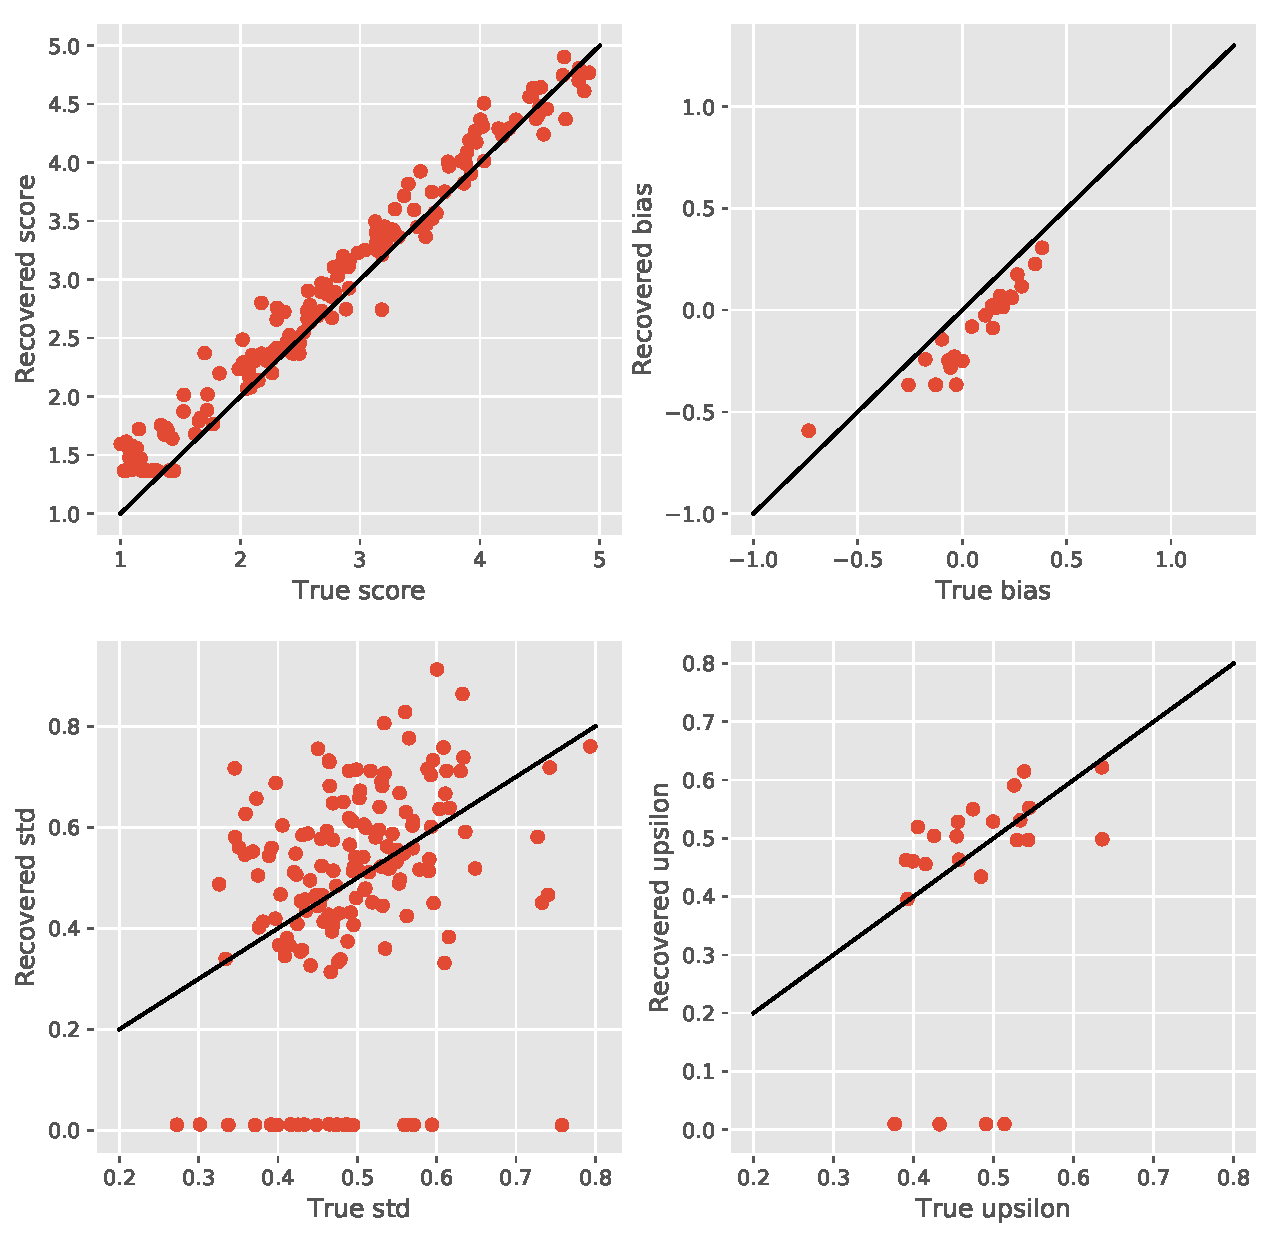
\includegraphics[width=0.6\linewidth]{mlenorm}
\end{center}
\end{frame}

\begin{frame}{MAP - continuous}
\begin{center}
	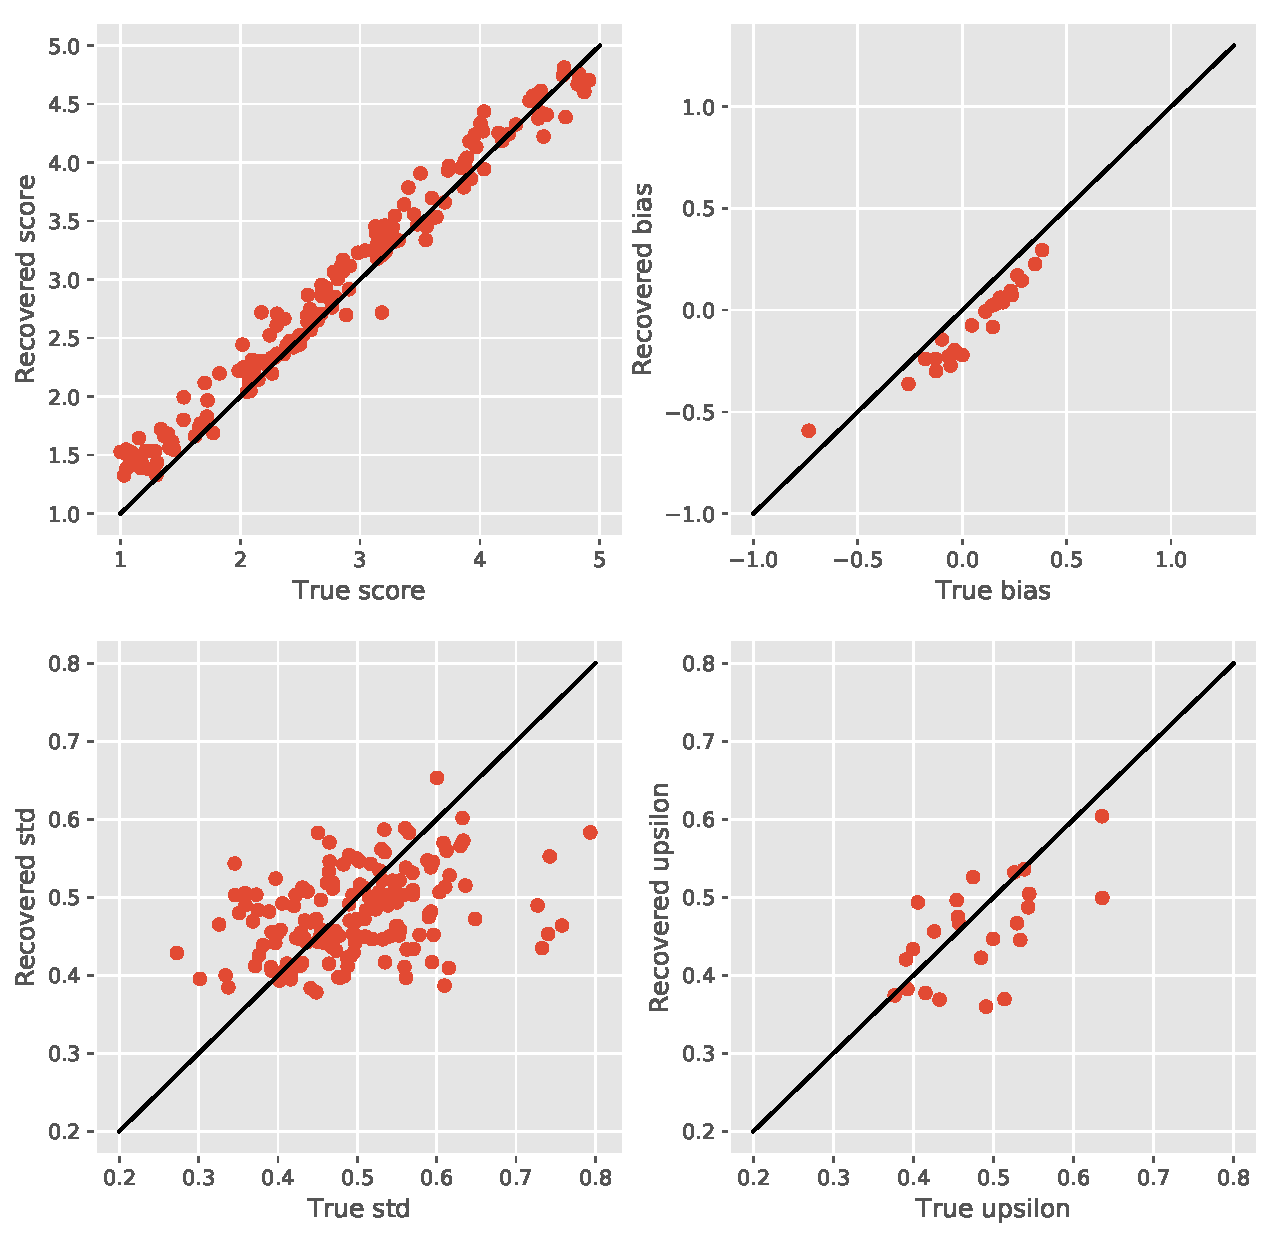
\includegraphics[width=0.6\linewidth]{mapnorm}
\end{center}
\end{frame}



\begin{frame}{MLE - quantized}
	\begin{center}
		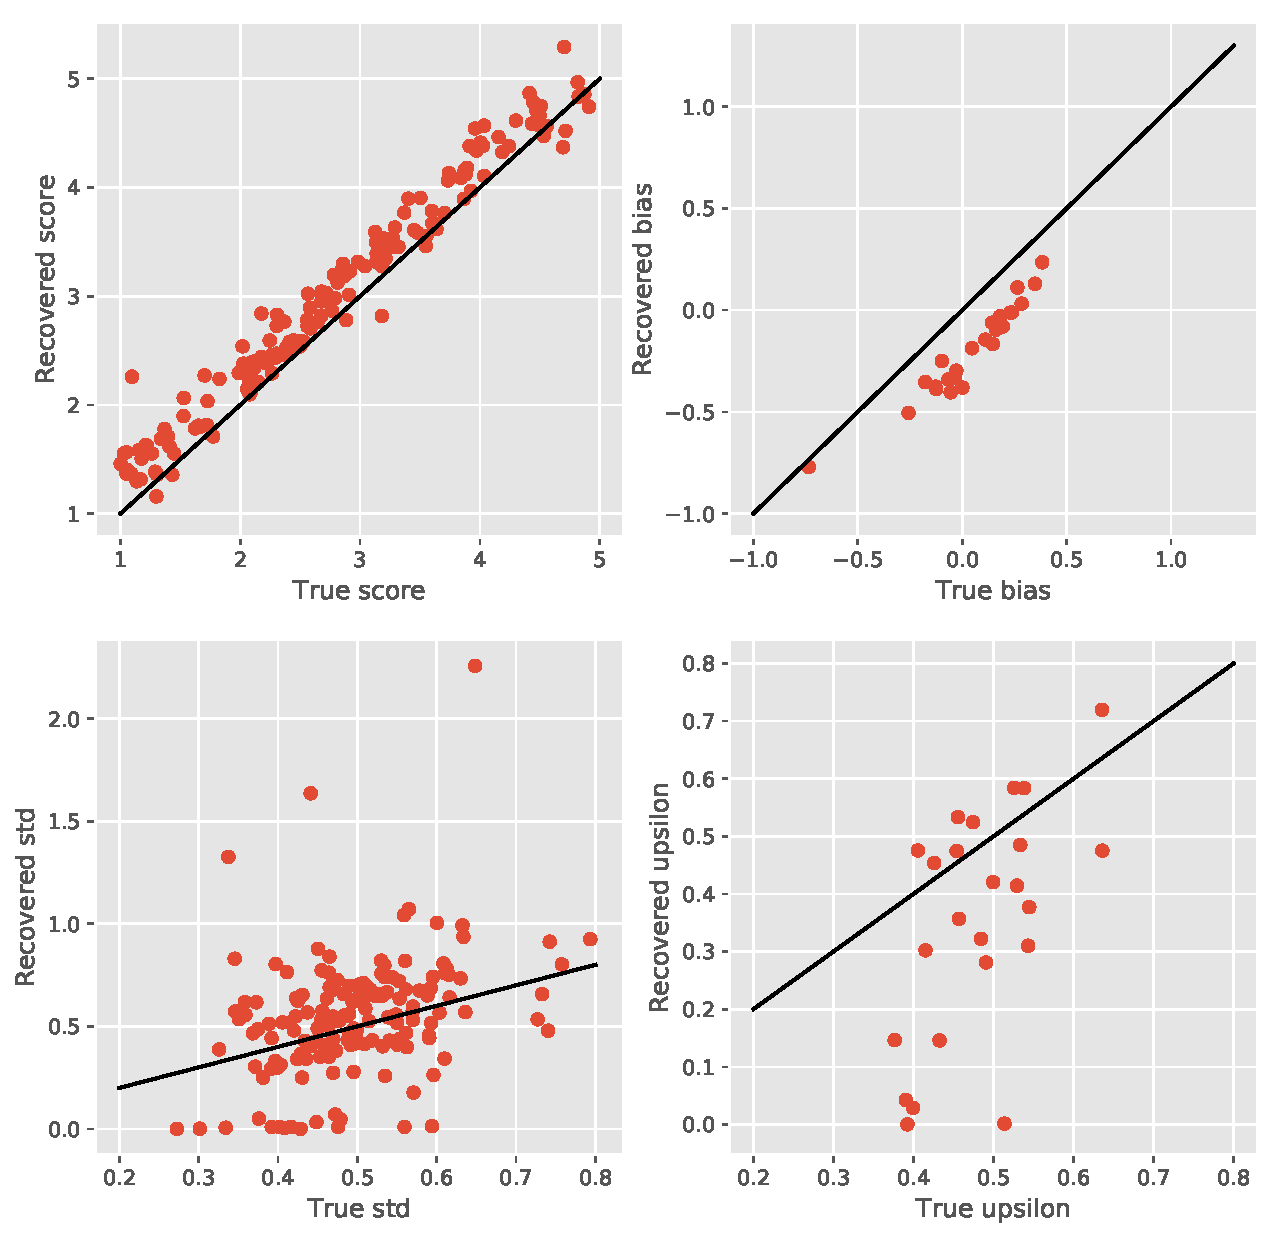
\includegraphics[width=0.6\linewidth]{mlequnta}
	\end{center}
\end{frame}
\begin{frame}{MAP - quantized}
\begin{center}
	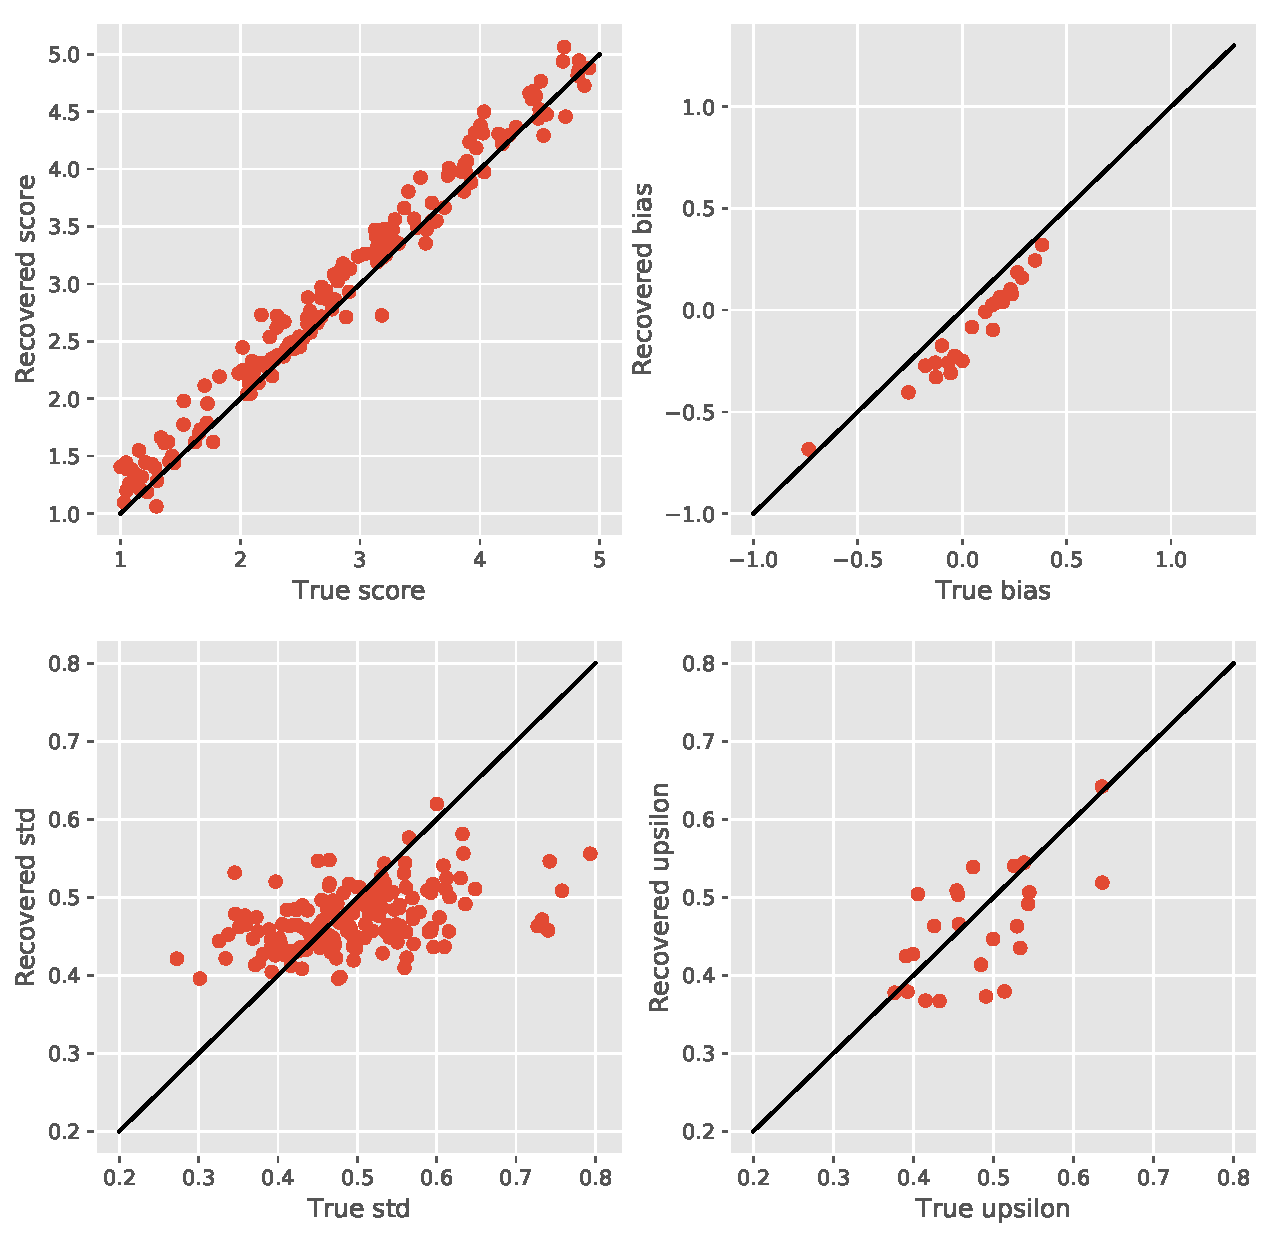
\includegraphics[width=0.6\linewidth]{mapquanta}
\end{center}
\end{frame}

\begin{frame}{Summary}
\begin{enumerate}
	\item MAP as a simple extension of MLE
	\item TensorFlow Probability allows fitting quantized distribution
	\item Optimization poses numerical problems 
	\item Next step: MCMC for full posterior distribution (confidence intervals) 
\end{enumerate}
\end{frame}
	
\end{document}